\documentclass[british]{article}
\usepackage[T1]{fontenc}
\usepackage[latin9]{inputenc}
\usepackage{geometry}
\geometry{verbose,tmargin=3.5cm,bmargin=3.5cm,lmargin=3cm,rmargin=3cm}
\usepackage{array}
%\usepackage{multirow}
\usepackage{amstext}
\usepackage{graphicx}
\usepackage{color}
\usepackage{caption}
%\usepackage{subfigure}

\newcommand{\tabincell}[2]{\begin{tabular}{@{}#1@{}}#2\end{tabular}}

\newcommand{\mytablefontsize}{7pt}
\newcommand{\mytablebaselineskip}{0.7}
\newcommand{\mytabcolsep}{3pt}

\newcommand{\medianInterval}[1]{}


\makeatletter

%%%%%%%%%%%%%%%%%%%%%%%%%%%%%% LyX specific LaTeX commands.
%% Because html converters don't know tabularnewline
\providecommand{\tabularnewline}{\\}

%%%%%%%%%%%%%%%%%%%%%%%%%%%%%% User specified LaTeX commands.

\title{Experimental Reports for \emph{Sparkle} }
\author{ \emph{Sparkle} }

\makeatother

\usepackage{babel}
\begin{document}
\maketitle %


\section{Introduction}
\label{sec:Introduction}

\emph{Sparkle} \cite{Hoos15} is a Programming by Optimisation (PbO) \cite{Hoos12} multi-agent problem-solving platform, and would provide many algorithm optimisation techniques (such as automated algorithm configuration, portfolio-based algorithm selection, etc) to light your solvers. 

This is the automatically generated report by \emph{Sparkle}, and this report is to present experimental results for solvers and instance classes submitted to \emph{Sparkle}.


\section{Experimental Preliminaries}
\label{sec:Experimental_Preliminaries}

In this section, we present the experimental preliminaries, including the list of solvers, the list of feature extractors, the list of instance classes, information about experimental setup and the information about how to construct a portfolio-based algorithm selector in \emph{Sparkle}.

\subsection{Solvers}
\label{sec:Solvers}
There are 4 solver(s) submitted in \emph{Sparkle}, and the list of solvers are given as follows.


\begin{enumerate} 
\item \textbf{PbO-CCSAT-FAC}
\item \textbf{PbO-CCSAT-SMT-QF-BV}
\item \textbf{Lingeling\textunderscore wrapper\textunderscore sparkle}
\item \textbf{PbO-CCSAT-PTN}

\end{enumerate}


\subsection{Feature Extractors}
\label{sec:Feature_Extractors}
There are 1 feature extractor(s) submitted in \emph{Sparkle}, and list of feature extractors are given as follow.

\begin{enumerate}
\item \textbf{SAT-features-competition2012\textunderscore sparkle}

\end{enumerate}

\subsection{Instance Classes}
\label{sec:Instance_Classes}
There are 1 instance class(es) submitted in \emph{Sparkle}, and the list of instance classes are given as follows.

\begin{enumerate}
\item \textbf{PTN-7824\textunderscore Train}, number of instances: 11

\end{enumerate}

\subsection{Experimental Setup}
\label{sec:Experimental_Setup}

\textbf{Feature computation:} We use all the feature extractors which are presented above to compute the feature vector for each instance. Each feature extractor will compute a feature vector for each instance. The final feature vector is the combination of all computed feature vectors. The cutoff time for feature vector computation on each instance is set to 90 seconds.

\textbf{Performance computation:} Each solver will run one time on each instance. The cutoff time for each performance computation run is set to 50 seconds.

\subsection{Constructing Portfolio-Based Algorithm Selector}
\label{sec:Portfolio}

\emph{Sparkle} runs all the feature extractors to compute the feature vector for each instance, and store the resulting the feature data in the system. Also, \emph{Sparkle} runs all the solvers to solve each instance, and store the resulting the performance data in the system. After the feature-related and the performance-related experiments done, by utilizing the computed feature data and performance data, \emph{Sparkle} uses \emph{AutoFolio} \cite{LinEtAl15} to automatically construct a portfolio-based algorithm selector for \emph{Sparkle}.

\section{Experimental Results}
\label{sec:Experimental_Results}

In this section, the related experimental results in \emph{Sparkle} are presented and analysed.

\subsection{PAR10 Ranking List}
\label{sec:PAR10_Ranking}

The ranking list with regards to the penalised average runtime (PAR10) for solvers is given as follows.

\begin{enumerate}
\item \textbf{Solvers/PbO-CCSAT-PTN}, PAR10: 3.06272727273
\item \textbf{Solvers/PbO-CCSAT-FAC}, PAR10: 93.27
\item \textbf{Solvers/PbO-CCSAT-SMT-QF-BV}, PAR10: 139.378181818
\item \textbf{Solvers/Lingeling\textunderscore wrapper\textunderscore sparkle}, PAR10: 500.0

\end{enumerate}

Also, PAR10 for the Virtual Best Solver \emph{VBS}, i.e., the perfect portfolio selector, and the actual portfolio selector in \emph{Sparkle} is given as follows.

\begin{itemize}
\item \textbf{\emph{VBS}}, PAR10: 3.04727272727
\item \textbf{Actual Portfolio Selector in \emph{Sparkle}}, PAR10: 3.06272727273
\end{itemize}

\subsection{Marginal Contribution Ranking List}
\label{sec:Marginal_Contribution_Ranking}

\emph{Sparkle} uses the concept of marginal contribution \cite{XuEtAl12} to measure each solver's contribution to the \textbf{\emph{VBS}} and to the \textbf{actual portfolio selector in \emph{Sparkle}}. In this report, we uses the approach described in the literature \cite{FreEtAl16} to each solver's marginal contribution.

Solver ranking list via marginal contribution \cite{XuEtAl12} for solvers with regards to the \textbf{{\em VBS}} is given as follows.

\begin{enumerate} 
\item \textbf{PbO-CCSAT-PTN}, marginal contribution: 2.03823716493
\item \textbf{PbO-CCSAT-SMT-QF-BV}, marginal contribution: 7.72376192639e-05
\item \textbf{PbO-CCSAT-FAC}, marginal contribution: 0.0
\item \textbf{Lingeling\textunderscore wrapper\textunderscore sparkle}, marginal contribution: 0.0

\end{enumerate}

Solver ranking list via marginal contribution \cite{XuEtAl12} for solvers with regards to the \textbf{actual portfolio selector in \emph{Sparkle}} is given as follows.

\begin{enumerate} 
\item \textbf{PbO-CCSAT-PTN}, marginal contribution: 2.04192639709
\item \textbf{PbO-CCSAT-FAC}, marginal contribution: 0.0
\item \textbf{PbO-CCSAT-SMT-QF-BV}, marginal contribution: 0.0
\item \textbf{Lingeling\textunderscore wrapper\textunderscore sparkle}, marginal contribution: 0.0

\end{enumerate}


\subsection{Scatter Plot Analysis}

The empirical comparison between the actual portfolio selector in \emph{Sparkle} and single best solver (\emph{SBS}) is presented in Figure \ref{fig:sparkle_vs_sbs}
The empirical comparison between the actual portfolio selector in \emph{Sparkle} and \emph{VBS} is presented in Figure \ref{fig:sparkle_vs_vbs}.

%\begin{figure}[htbp]
%\begin{minipage}{0.5\linewidth}
%\noindent \begin{centering}
%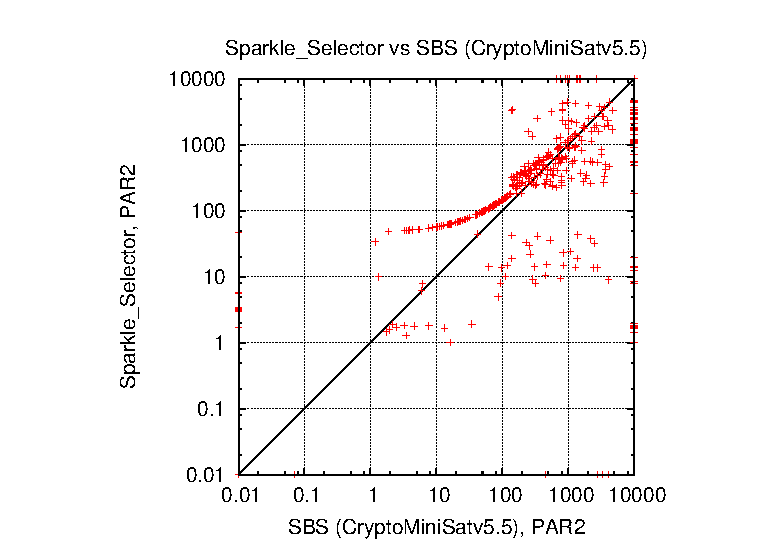
\includegraphics[width=0.6\textwidth]{figure_portfolio_selector_sparkle_vs_sbs}
%\par\end{centering}
%\caption{Empirical comparison between the actual portfolio selector in \emph{Sparkle} and \emph{SBS}.}\label{fig:sparkle_vs_sbs}
%\end{minipage}

%\begin{minipage}{0.5\linewidth}
%\noindent \begin{centering}
%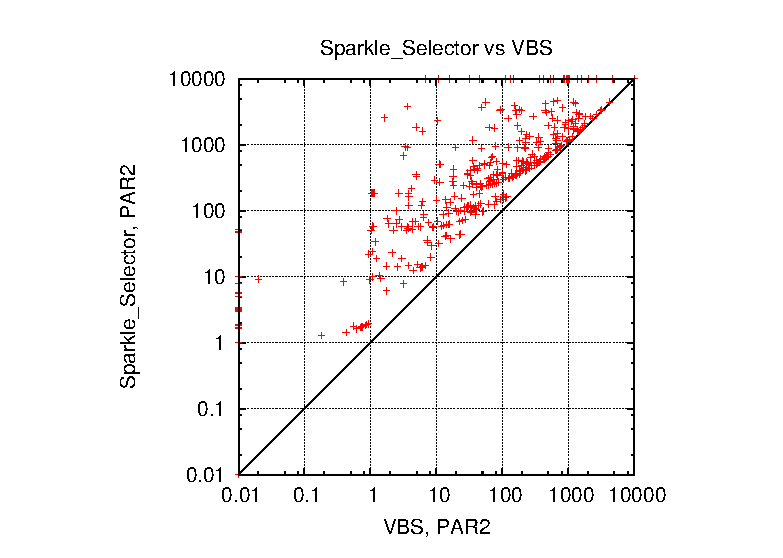
\includegraphics[width=0.6\textwidth]{figure_portfolio_selector_sparkle_vs_vbs}
%\par\end{centering}
%
%\end{minipage}
%\end{figure}

\begin{figure}[htbp]
\noindent \begin{centering}
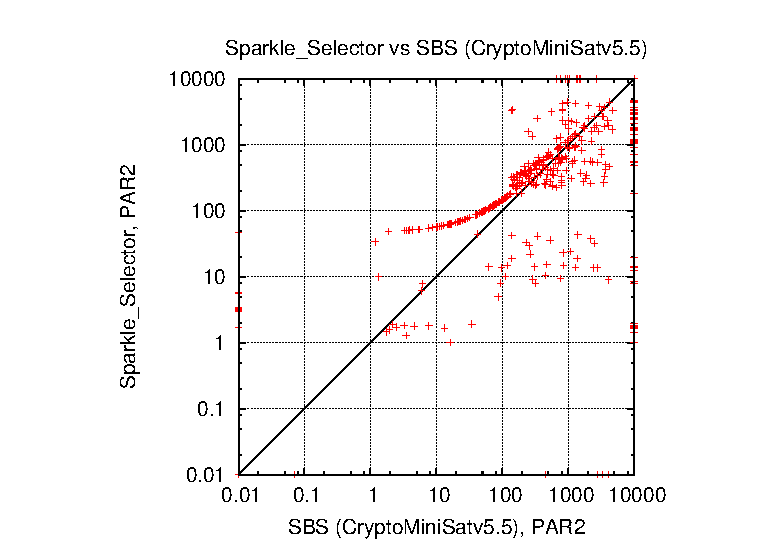
\includegraphics[width=0.6\textwidth]{figure_portfolio_selector_sparkle_vs_sbs}
% \includegraphics[width=0.8\textwidth]{fittedModels}
\par\end{centering}

\caption{Empirical comparison between the actual portfolio selector in \emph{Sparkle} and \emph{SBS}.}\label{fig:sparkle_vs_sbs}
\end{figure}

\begin{figure}[htbp]
\noindent \begin{centering}
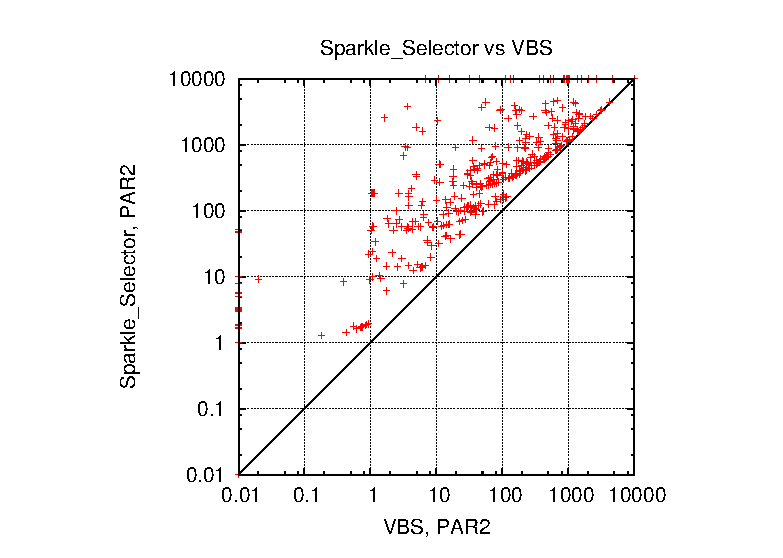
\includegraphics[width=0.6\textwidth]{figure_portfolio_selector_sparkle_vs_vbs}
% \includegraphics[width=0.8\textwidth]{fittedModels}
\par\end{centering}

\caption{Empirical comparison between the actual portfolio selector in \emph{Sparkle} and \emph{VBS}.}\label{fig:sparkle_vs_vbs}
\end{figure}



\bibliographystyle{plain}
\bibliography{Sparkle_Report}

\end{document}
